
%%Программная реализация (на языке Javascript) алгоритмов
%% генерации фонда оценочных средств по математике
\section{Планиметрия}
В это главе мы приводим вспомогательные функции и алгоритм написания шаблона по планиметрии
\subsection{Вспомогательные функции}
\subsubsection{Функции для работы с массивами}
\prototype[repeat]{Array}{permuteCyclic}
Возвращает массив после циклической перестановки.
В листинге \ref{lst:92} в строке \ref{line:permuteCyclic-1} функция используется для перестановки букв в названии параллелограмма, а в строке \ref{line:permuteCyclic-2} — в названии трапеции.

\begin{lstlisting}
    let array = [1, 2, 3, 4, 5];

    array.permuteCyclic(1);
    // [5, 1, 2, 3, 4]

    array.permuteCyclic(-2);
    // [3, 4, 5, 1, 2]

    array.permuteCyclic(0);
    // [1, 2, 3, 4, 5]
    \end{lstlisting}

\prototype{Array}{mt\_coordinatesOfIntersectionOfTwoSegments\\}
Возвращает координаты пересечения двух отрезков, задаваемых первыми парами точек из массива. Является вспомогательной для функции \texttt{arcBetweenSegments}.

\begin{lstlisting}[escapechar=|]
    let array = [{x:0,y:5},{x:-4,y:4},{x:1,y:10},{x:-3,y:6}];

    array.mt_coordinatesOfIntersectionOfTwoSegments()
    //{ x: -5.333333333333333, y: 3.666666666666667, status: false }
    //Если status — false, отрезки не пересекаются, но прямые проходящие через них пересекаются в точке {x,y}

    array = [{x:0,y:5},{x:-4,y:4},{x:1,y:1},{x:-3,y:6}];
    array.mt_coordinatesOfIntersectionOfTwoSegments()
    //{ x: -1.8333333333333333, y: 4.541666666666667, status: true }
    //Если status — true, отрезки пересекаются в точке {x,y}
        
\end{lstlisting}

\prototype[separator]{Array}{shuffleJoin}
Перемешивает и соединяет массив с разделителем \texttt{separator}. \texttt{separator} по умолчанию пустая строка. Функция используется в \ref{lst:3011}
в строке \ref{line:shuffleJoin} для отображения условий задачи в случайном порядке.

\begin{lstlisting}
    let array = ['A', 'B', 'C', 'D',];
    array.shuffleJoin();
    //ADBC

    array.shuffleJoin('; ');
    //C; D; B; A 
\end{lstlisting}

\prototype[separator]{Array}{joinWithConjunction}
Соединяет массив запятыми и соединяет два последних элемента союзом «и».

\begin{lstlisting}
    let array = ['A', 'B', 'C', 'D',];

    array.joinWithConjunction();
    //A, B, C и D
\end{lstlisting}

\subsubsection{Функции для работы с числами}
\prototype{Number}{perfectCubicMultiplier}
Возвращает максимальный делитель данного числа, куб которого также является делителем данного числа.

\begin{lstlisting}
    let number = 81;

    number.perfectCubicMultiplier()
    //3

    number = 36;
    number.perfectCubicMultiplier()
    //1

    number = -27;
    number.perfectCubicMultiplier()
    //3
\end{lstlisting}

\prototype[p1, p2]{Number}{texcbrt}
TeX-представление кубического корня из данного числа.\\
Если данное число - полный куб, то корень из числа.\\
Если \texttt{p1}, то из-под корня будут вынесены возможные множители.\\
Если \texttt{p1}, \texttt{p2} и из-под корня выносится единица, то она будет опущена\\

\includegraphics[width=0.8\textwidth]{texcbrt.png}

\subsubsection{Функции для работы с canvas}
\prototype[vertex,\\ fillStyle]{CanvasRenderingContext2D}{drawSection}
Заполняет область цветом \texttt{fillStyle} по вершинам из массива \texttt{vertex}.

\begin{lstlisting}
    let paint1 = function(ctx) {
        let h = 400;
        let w = 400;
        ctx.drawCoordinatePlane(w, h, {
            hor: 1,
            ver: 1
        }, {
            x1: '1',
            y1: '1',
            sh1: 16,
        },30);
        ctx.scale(30, -30);
        ctx.drawSection([[1, 3],[-3, 0],[-2, -2],[1, -1],[5, 1],[4, 4],[3, 2]]);

        ctx.drawSection([[-2, 0],[-1, 1],[-4, 3],[-1, 5],[1, 1],[5, 2],[4, -6],[0, 0],[-4, -2],]);
    };
    \end{lstlisting}
    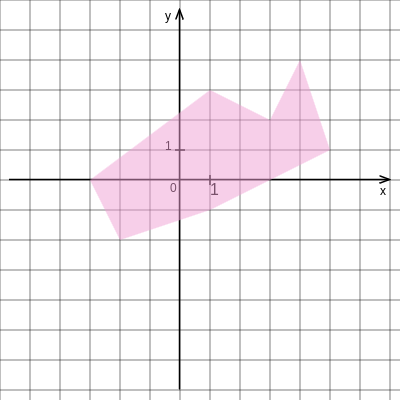
\includegraphics[width=0.4\textwidth]{drawSection-1.png}
    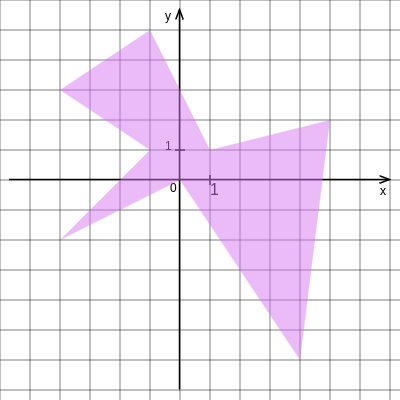
\includegraphics[width=0.4\textwidth]{drawSection-2.png}

\prototype[x, y,\\ angle, length]{CanvasRenderingContext2D}{drawLineAtAngle}
Рисует отрезок длины \texttt{length} под углом angle ( в радианах). Пример использования можно найти в листинге \ref{lst:2069} в строках \ref{line:drawLineAtAngle-1} и \ref{line:drawLineAtAngle-2} (применяется для отрисовки биссектрисы). 

\prototype[x1, y1, x2, y2, length, quantity]{CanvasRenderingContext2D}{strokeInMiddleOfSegment\\}
Ставит штрихи длины \texttt{length} на середине отрезка перпендикулярно ему. Функция используется в листинге \ref{lst:2069} в строках \ref{line:strokeInMiddleOfSegment-1}-\ref{line:strokeInMiddleOfSegment-2} для обозначения равных по длине сторон треугольника.

\prototype[x, y, angle, letter, length, maxLength]{CanvasRenderingContext2D}{markSegmentWithLetter\\}
Вспомогательная функция для отрисовки текста около некоторого отрезка.

\prototype[x1, y1, x2, y2, letter, length, maxLength]{CanvasRenderingContext2D}{signSegmentInMiddle\\}
Рисует строку \texttt{letter} на середине отрезка. В листинге \ref{lst:27193} в строках \ref{line:signSegmentInMiddle-1} - \ref{line:signSegmentInMiddle-2} функция используется для отображения длин рёбер многогранника.

\prototype[coordinates, radius]{CanvasRenderingContext2D}{arcBetweenSegments\\}
Рисует знак угла между двумя отрезками в месте их пересечения. \texttt{coordinates} - массив вида \texttt{[x1, y1, x2, y2]}.

\begin{lstlisting}
    let paint1 = function(ctx) {
        let h = 400;
        let w = 400;
        ctx.drawCoordinatePlane(w, h, {
            hor: 1,
            ver: 1
        }, {
            x1: '1',
            y1: '1',
            sh1: 16,
        }, 30);
        ctx.scale(30, -30);

        ctx.lineWidth = 2 / 30;
        ctx.drawLine(1, 5, 3, -2);
        ctx.drawLine(3, -2, 5, -3);
        ctx.arcBetweenSegments([1, 5, 3, -2, 5, -3], 2);

        ctx.drawLine(2, -5, -4, -2);
        ctx.drawLine(1, -2, -3, -6);
        ctx.arcBetweenSegments([2, -5, -4, -2,  -3, -6,1, -2,], 1);

        ctx.drawLine(1, 5, 1, -2);
		ctx.drawLine(1, -2, 5, -2);
		ctx.strokeStyle = om.secondaryBrandColors.iz();
		ctx.arcBetweenSegments([1, 5, 1, -2, 5, -2], 3);

    };
\end{lstlisting}

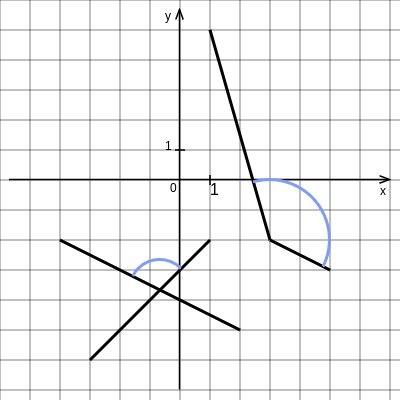
\includegraphics[width=0.4\textwidth]{arcBetweenSegments-1.png}    
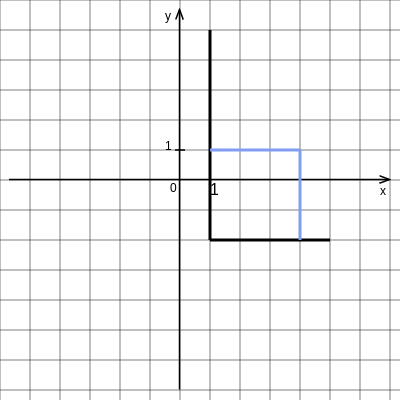
\includegraphics[width=0.4\textwidth]{arcBetweenSegments-2.png}    

\prototype[coordinates, radius, number, step]{CanvasRenderingContext2D}{arcBetweenSegmentsCount\\}
Рисует знак угла между двумя отрезками в месте их пересечения \texttt{number} раз с отступом \texttt{step}. В листинге \ref{lst:27764} в строках \ref{line:arcBetweenSegmentsCount-1} - \ref{line:arcBetweenSegmentsCount-2} используется для обозначения двух равных углов.

\prototype[x, y, radiusX, radiusY, rotation, startAngle, endAngle,\\ anticlockwise]{CanvasRenderingContext2D}{drawEllipse\\}
Рисует эллипс.

\prototype[x, y, radius, startAngle, endAngle, anticlockwise]{CanvasRenderingContext2D}{drawArc\\}
Рисует дугу.

\subsubsection{Элементы декларативного программирования}

\textbf{Определение.} Декларативное программирование — парадигма программирования, в которой задается спецификация решения задачи, то есть описывается конечный результат, а не способ его достижения.

Во время разработки шаблонов по теме «Графики функции» требовалось много раз переопределять коэффициенты функций через циклы 
\texttt{while} или \texttt{do\dots while}, пока они не начнут соответствовать заданным условиям (видимость графика, сливание его с осями, видимость целых точек). Это часто приводило к бесконечной работе шаблона, при этом сложно было определить, какое условие не выполняется.

Для этого было разработано окружение \texttt{retryWhileUndefined} для шаблонов, которое бы перезапускало их не более \texttt{maxIterations} раз, если одно из условий не удовлетворено. 

\function{retryWhileUndefined}{theFunction, maxIterations}

Но всё равно было тяжело определить, почему шаблон перезапускается. Для этого было разработано более совершенное окружение \texttt{retryWhileError}, которое не только могло бы ограничивать количество перезапусков, но и фиксировать, какие проверки не были пройдены и выводить их на экран (ошибки видны только для разработчика при отладке).

\function{retryWhileError}{theFunction, maxIterations,maxCollectedErrors}

Для окружения были написаны функции-утверждения, которые имеют структуру : условие не выполнено - записать ошибку - перезапустить шаблон. Если максимальное количество повторений достигнуто, то вывести накопившиеся ошибки и количество их появлений. 

\function{genAssert}{condition, message}
    Если условие \texttt{condition} ложно, то шаблон перезапускается. 

\function{genAssertNonempty}{array, message}
    Если массив \texttt{array} пуст, то шаблон перезапускается.

\function{genAssertZ1000}{number, message}
    Если число \texttt{number} имеет более 3 знаков после запятой, то шаблон перезапускается.
    
\function{genAssertIrreducible}{numerator, denominator, message}
    Если дробь \texttt{numerator/denominator} сократима, то шаблон перезапускается.

\function{genAssertSaneDecomposition}{number, maxFactor, message}
    Если \texttt{number} число не раскладывается на простые множители, не более одного из которых превосходит \texttt{maxFactor}, то шаблон перезапускается. 

\subsection{Этапы разработки шаблона со вспомогательным чертежом по теме «Планиметрия»}

Для примера возьмём задание №19416~\cite{egemath}.
\\
\textbf{Задача №19376.}
В треугольнике $ABC$ известно, что ${AC=BC}$, $AB=16$, $AH$ — высота, $BH=4$. Найдите косинус угла $BAC$.\\ 

Заготовка шаблона имеет вид.

\lstinputlisting[]{code/109_1.js}

\begin{enumerate}
    \item Начнём с отрисовки чертежа для задания. Отметим стороны треугольника так, чтобы он лежал в центре холста, а до краёв оставалось 10-20px. При отрисовке используем функцию \texttt{drawLine}. Добавим высоту 
    \lstinputlisting[]{code/109_2.js} 
    \item Добавим на рисунок штрихи, указывающие на равенство сторон и обозначение прямого угла при помощи функций strokeInMiddleOfSegment и arcBetweenSegments соответственно. И подпишем вершины и точку перпендикуляра. Добавим модификатор \texttt{NAtask.modifiers.variativeABC(vertices)}, который заменяет все буквы в задании на случайные.
    %TODO: пояснить за параметр

    \lstinputlisting[]{code/109_3.js} 
    \item Теперь добавим ответ в задание. Проверим при помощи \texttt{genAssertZ1000}, что ответ имеет не более трёх знаков после запятой (если иначе шаблон запускается заново). Поместим все буквы и числа в \$\dots\$. Все условия из задачи преобразуем в массив и соединим случайным образом с помощью функции \texttt{shuffleJoin}.
    \lstinputlisting[]{code/109_4.js} 
\end{enumerate}

